
\documentclass[11pt,a4paper]{article}
\usepackage[utf8]{inputenc}
\usepackage[english]{babel}
\usepackage{amsmath}
\usepackage{amsfonts}
\usepackage{amssymb}
\usepackage{graphicx}
\usepackage{float}
\usepackage{geometry}
\usepackage{fancyhdr}
\usepackage{booktabs}
\usepackage{subcaption}
\usepackage{hyperref}

\geometry{margin=2.5cm}
\pagestyle{fancy}
\fancyhf{}
\rhead{Methods in Computational Neuroscience}
\lhead{Homework 5 - Drift-Diffusion Model}
\cfoot{\thepage}

\title{Decision Making: Studying the Drift-Diffusion Model For Perceptual Decision Making}
\author{Sepehr SAEEDPOUR}
\date{\today}

\begin{document}

\maketitle

\section{Introduction}

% The drift-diffusion model (DDM) is a fundamental framework for understanding perceptual decision-making processes in neuroscience. This model describes how evidence accumulates over time until a decision threshold is reached, making it particularly relevant for two-alternative forced choice (2AFC) tasks. In this report, we analyze the DDM through computational simulations, examining how various parameters influence decision outcomes and reaction times.

The drift-diffusion model (DDM) is a fundamental framework for understanding perceptual decision-making processes in neuroscience. This model describes how evidence accumulates over time until a decision threshold is reached, making it particularly relevant for two-alternative forced choice (2AFC) tasks.
The DDM has its roots in the 1970s, when Roger Ratcliff introduced it to model two-choice decision-making tasks. Building upon earlier concepts of evidence accumulation, Ratcliff's model provided a quantitative framework to explain both the accuracy and reaction time distributions observed in such tasks. Over the years, the DDM has been extensively validated and refined, becoming a cornerstone in cognitive psychology and neuroscience for modeling decision-making processes.

In this report, we analyze the DDM through computational simulations, examining how various parameters influence decision outcomes and reaction times.

% The mathematical formulation of the drift-diffusion model is given by:

% \begin{equation}
% \frac{dx(t)}{dt} = (I_A - I_B) + \sigma\eta(t)
% \label{eq:ddm}
% \end{equation}

% where $x(t)$ represents the decision variable, $I_A$ and $I_B$ are the decision inputs favoring alternatives A and B respectively, $\sigma$ is the noise magnitude, and $\eta(t)$ is Gaussian white noise with unit standard deviation. A decision for alternative A is made when $x(t) \geq \mu$, while a decision for alternative B occurs when $x(t) \leq -\mu$, where $\mu$ represents the decision threshold.


\section{Results}

\subsection{Simulate the dynamics}

We simulated the drift-diffusion process for 10 trajectories using the parameters $I_A = 0.95$, $I_B = 1.0$, $\sigma = 7$, and $\mu = 20$. All simulations started from the initial condition $x_0 = 0$ and were run for a maximum of 10,000 time steps.
The Euler-Maruyama method was used for numerical integration with a time step of $dt = 0.1$.

For the stochastic differential equation, the discrete update rule is:
\begin{equation}
x_{t+1} = x_t + (I_A - I_B) \cdot dt + \sigma \sqrt{dt} \cdot \xi_t
\end{equation}

where $\xi_t$ is a standard normal random variable.


% FIGURE PLACEHOLDER FOR QUESTION 1.1
\begin{figure}[H]
    \centering
    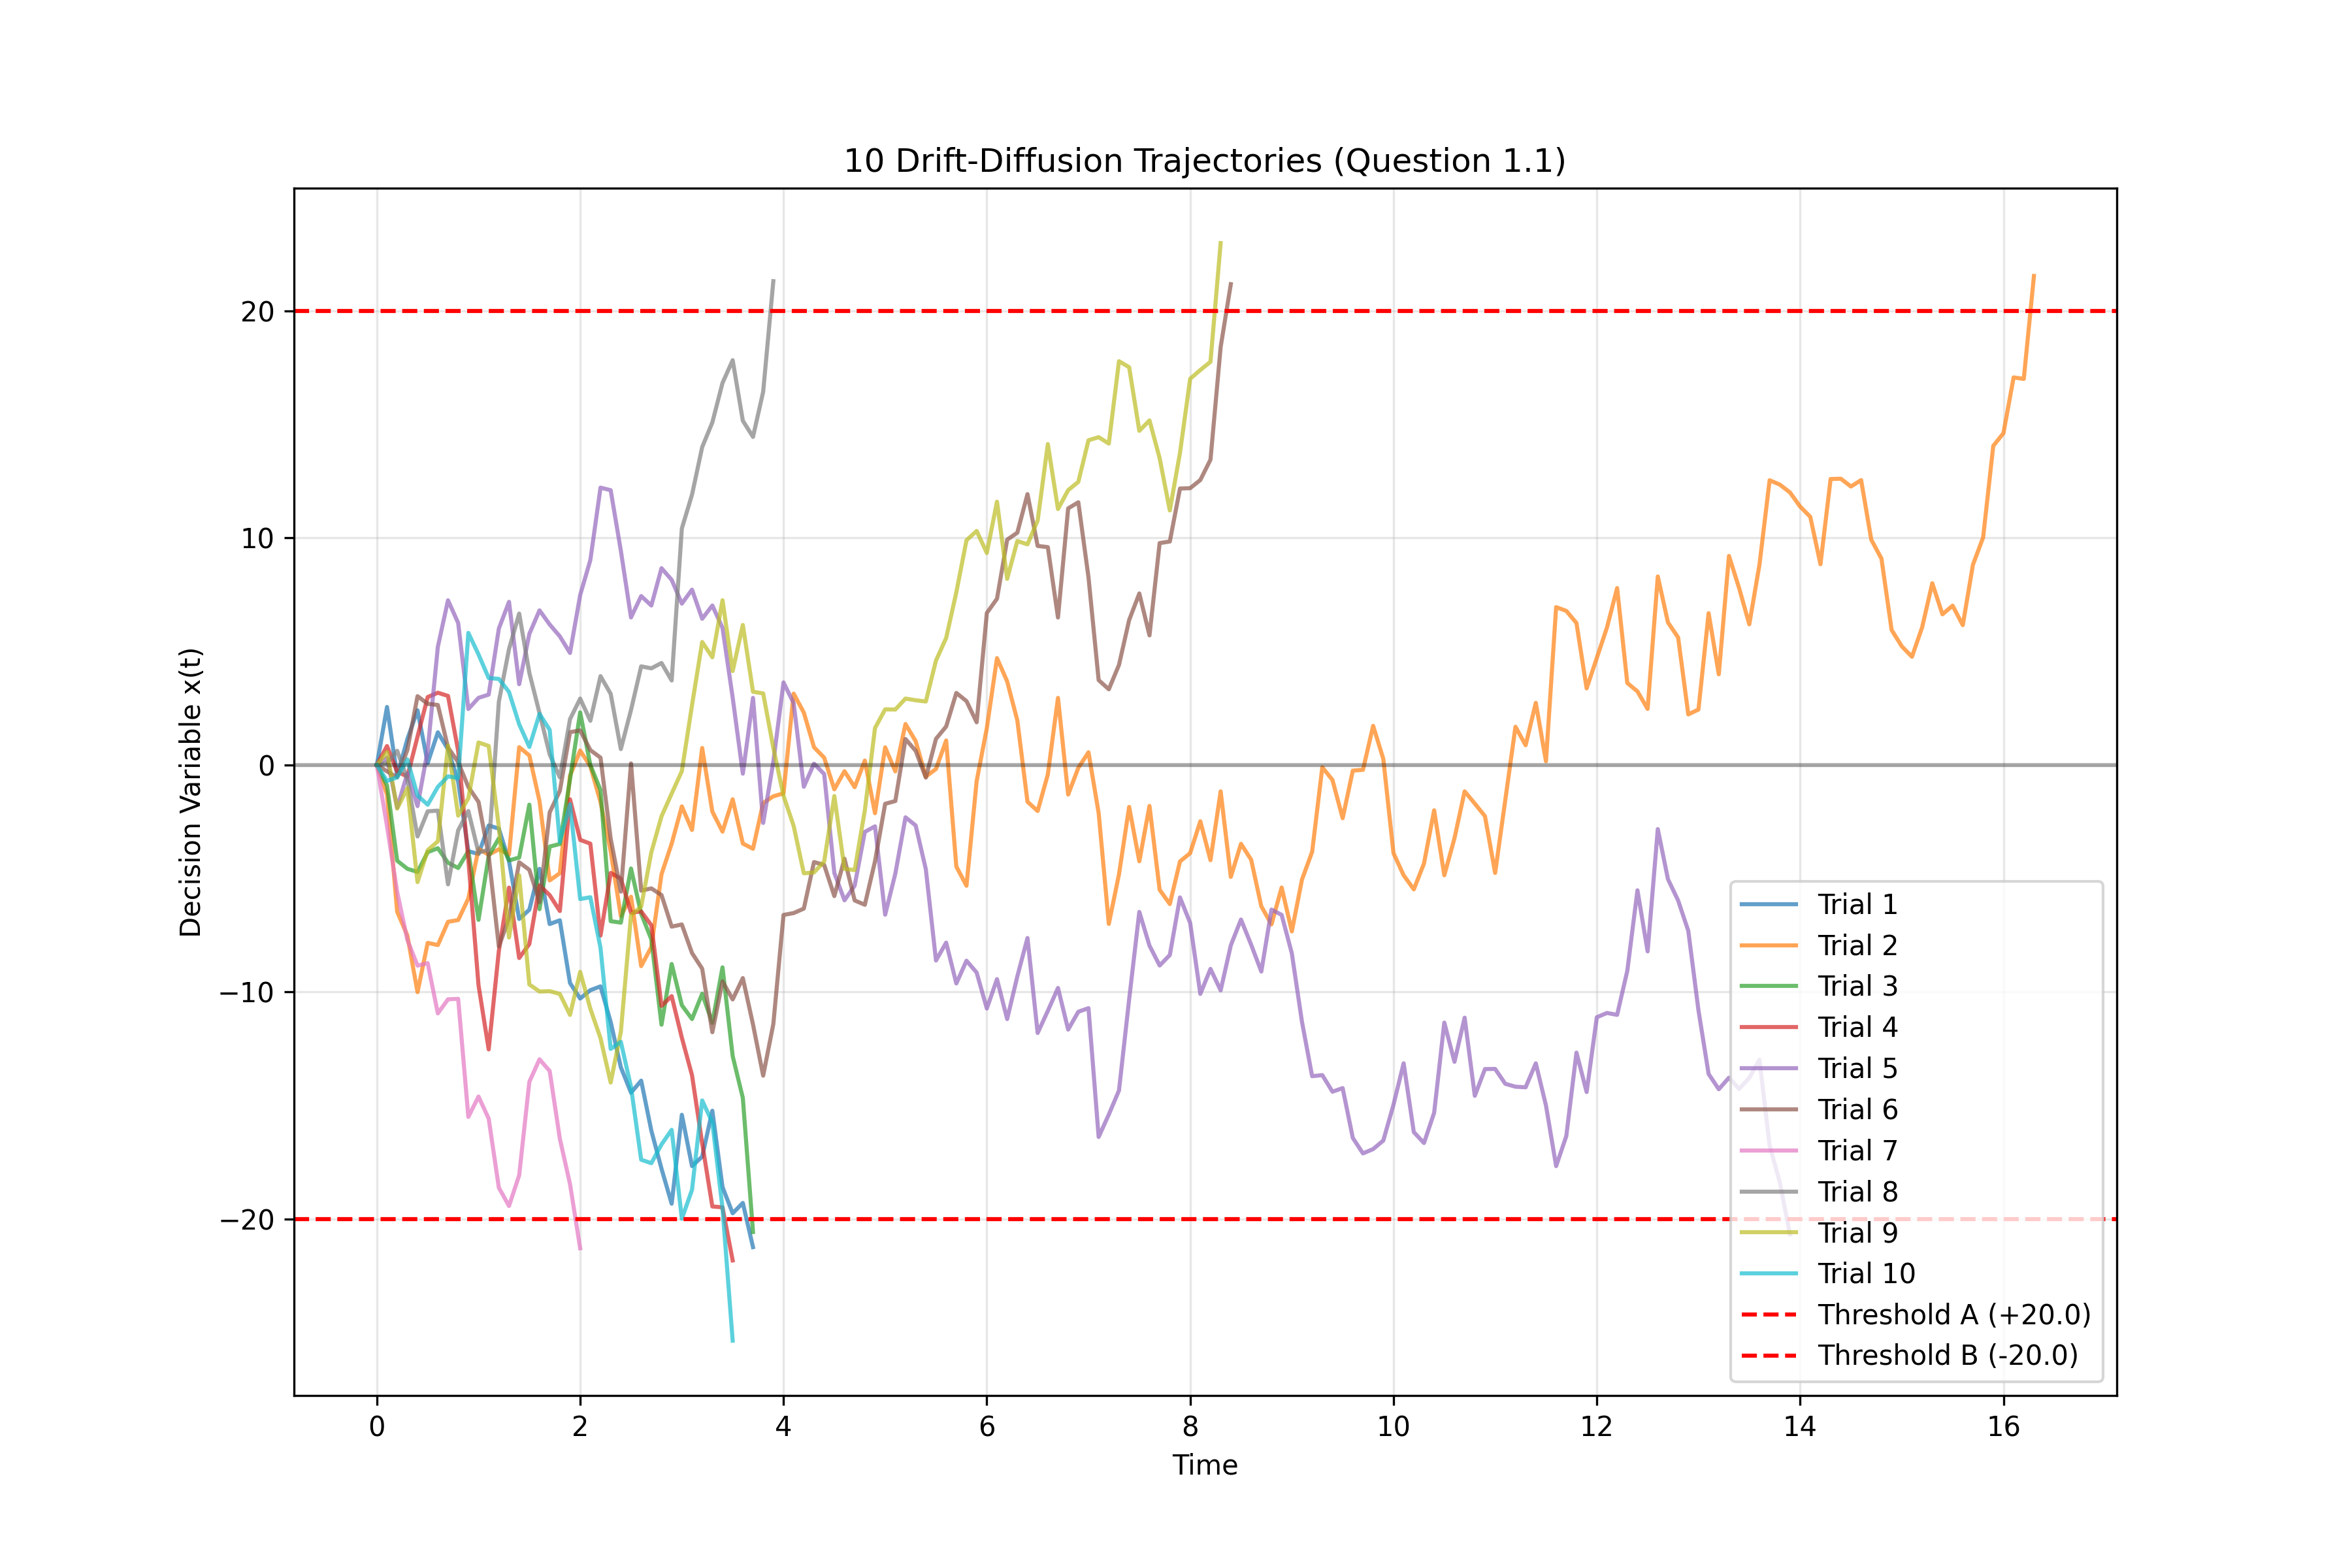
\includegraphics[width=0.6\textwidth]{ddm_trajectories_10.png}
    \caption{Ten trajectories of the drift-diffusion process. Red dashed lines indicate decision thresholds at $\pm 20$. Each trajectory shows the evolution of the decision variable $x(t)$ over time until a decision is reached or the maximum simulation time is exceeded.}
    \label{fig:trajectories}
\end{figure}

The trajectories demonstrate the stochastic nature of the decision-making process. Due to the negative evidence ($E = I_A - I_B = -0.05$), there is a slight bias toward decision B, though individual trajectories can still reach either threshold due to noise fluctuations.

\subsection{Store the outcomes}

From 1,000 simulation trials with identical parameters, we obtained the following outcome distribution:

% TABLE FOR OUTCOMES - You can fill in your actual numbers
\begin{table}[H]
    \centering
    \begin{tabular}{@{}lcc@{}}
        \toprule
        Outcome & Count  \\
        \midrule
        Decision A & 485  \\
        Decision B & 515 \\
        No Decision & 0 \\
        \bottomrule
    \end{tabular}
    \caption{Distribution of outcomes from 1,000 drift-diffusion simulations. The slight bias toward decision B reflects the negative evidence value. The results confirm the expected bias toward decision B due to the negative evidence ($E = -0.05$), while the presence of no-decision trials indicates that some trajectories failed to reach either threshold within the simulation time limit. }
    \label{tab:outcomes}
\end{table}

% The results confirm the expected bias toward decision B due to the negative evidence ($E = -0.05$), while the presence of no-decision trials indicates that some trajectories failed to reach either threshold within the simulation time limit.

\subsection{Vary the parameters}

\subsubsection*{Threshold Variation}

We investigated how the decision threshold $\mu$ affects outcome frequencies by varying $\mu$ from 1 to 100 while keeping other parameters constant ($I_A = 0.95$, $I_B = 1.0$, $\sigma = 7$).

% FIGURE PLACEHOLDER FOR THRESHOLD VARIATION
\begin{figure}[H]
    \centering
    % INSERT YOUR THRESHOLD VARIATION PLOT HERE
    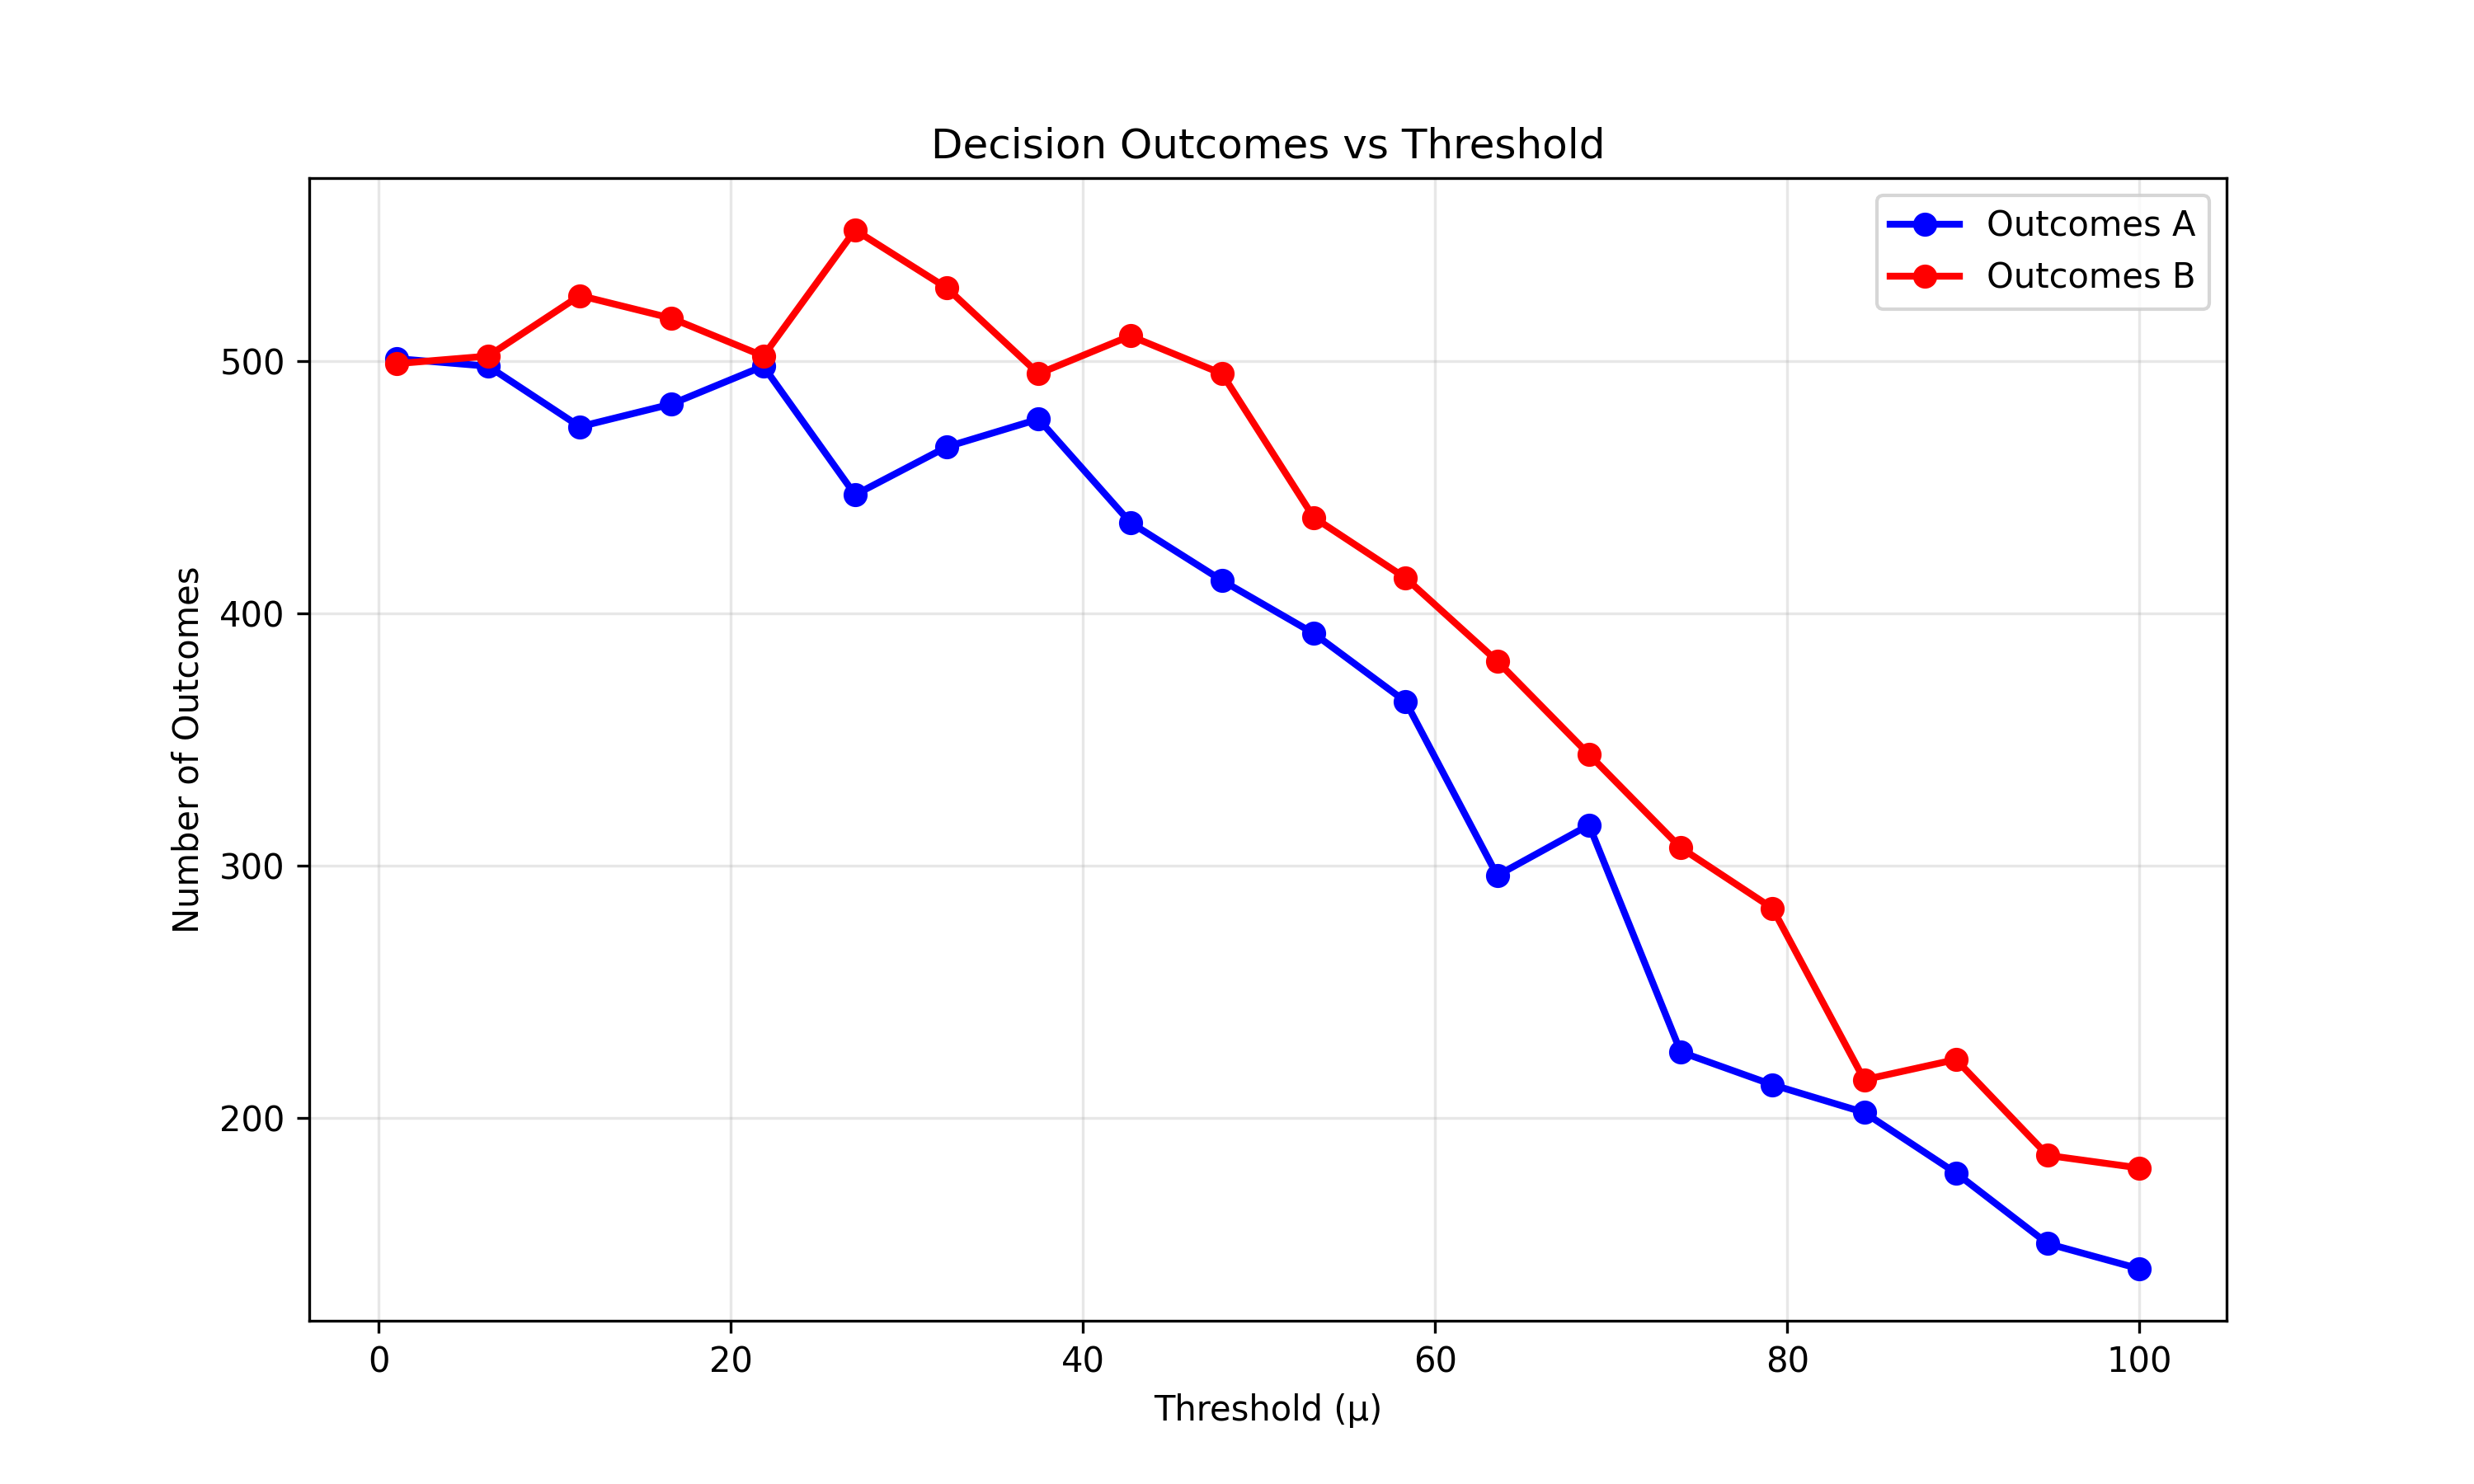
\includegraphics[width=0.6\textwidth]{ddm_threshold_variation.png}
    \caption{Effect of decision threshold $\mu$ on outcome frequencies. Higher thresholds require more accumulated evidence, leading to fewer total decisions but potentially higher accuracy.}
    \label{fig:threshold_variation}
\end{figure}

The analysis reveals that increasing the decision threshold leads to fewer overall decisions (more no-decision outcomes), longer decision times (representing a higher accuracy-speed trade-off), and maintained bias toward the favored alternative due to $E=-0.05$ (decision B in this case). 
% This demonstrates the fundamental speed-accuracy tradeoff in decision-making processes, where requiring more evidence before committing to a choice increases decision quality but at the cost of longer deliberation times.

\subsubsection*{Evidence Variation}

We examined how evidence strength $E = I_A - I_B$ influences decision bias by varying $E$ from -0.5 to 0.5 while maintaining $I_B = 1.0$, $\sigma = 7$, and $\mu = 20$.

% FIGURE PLACEHOLDER FOR EVIDENCE VARIATION
\begin{figure}[H]
    \centering
    % INSERT YOUR EVIDENCE VARIATION PLOT HERE
    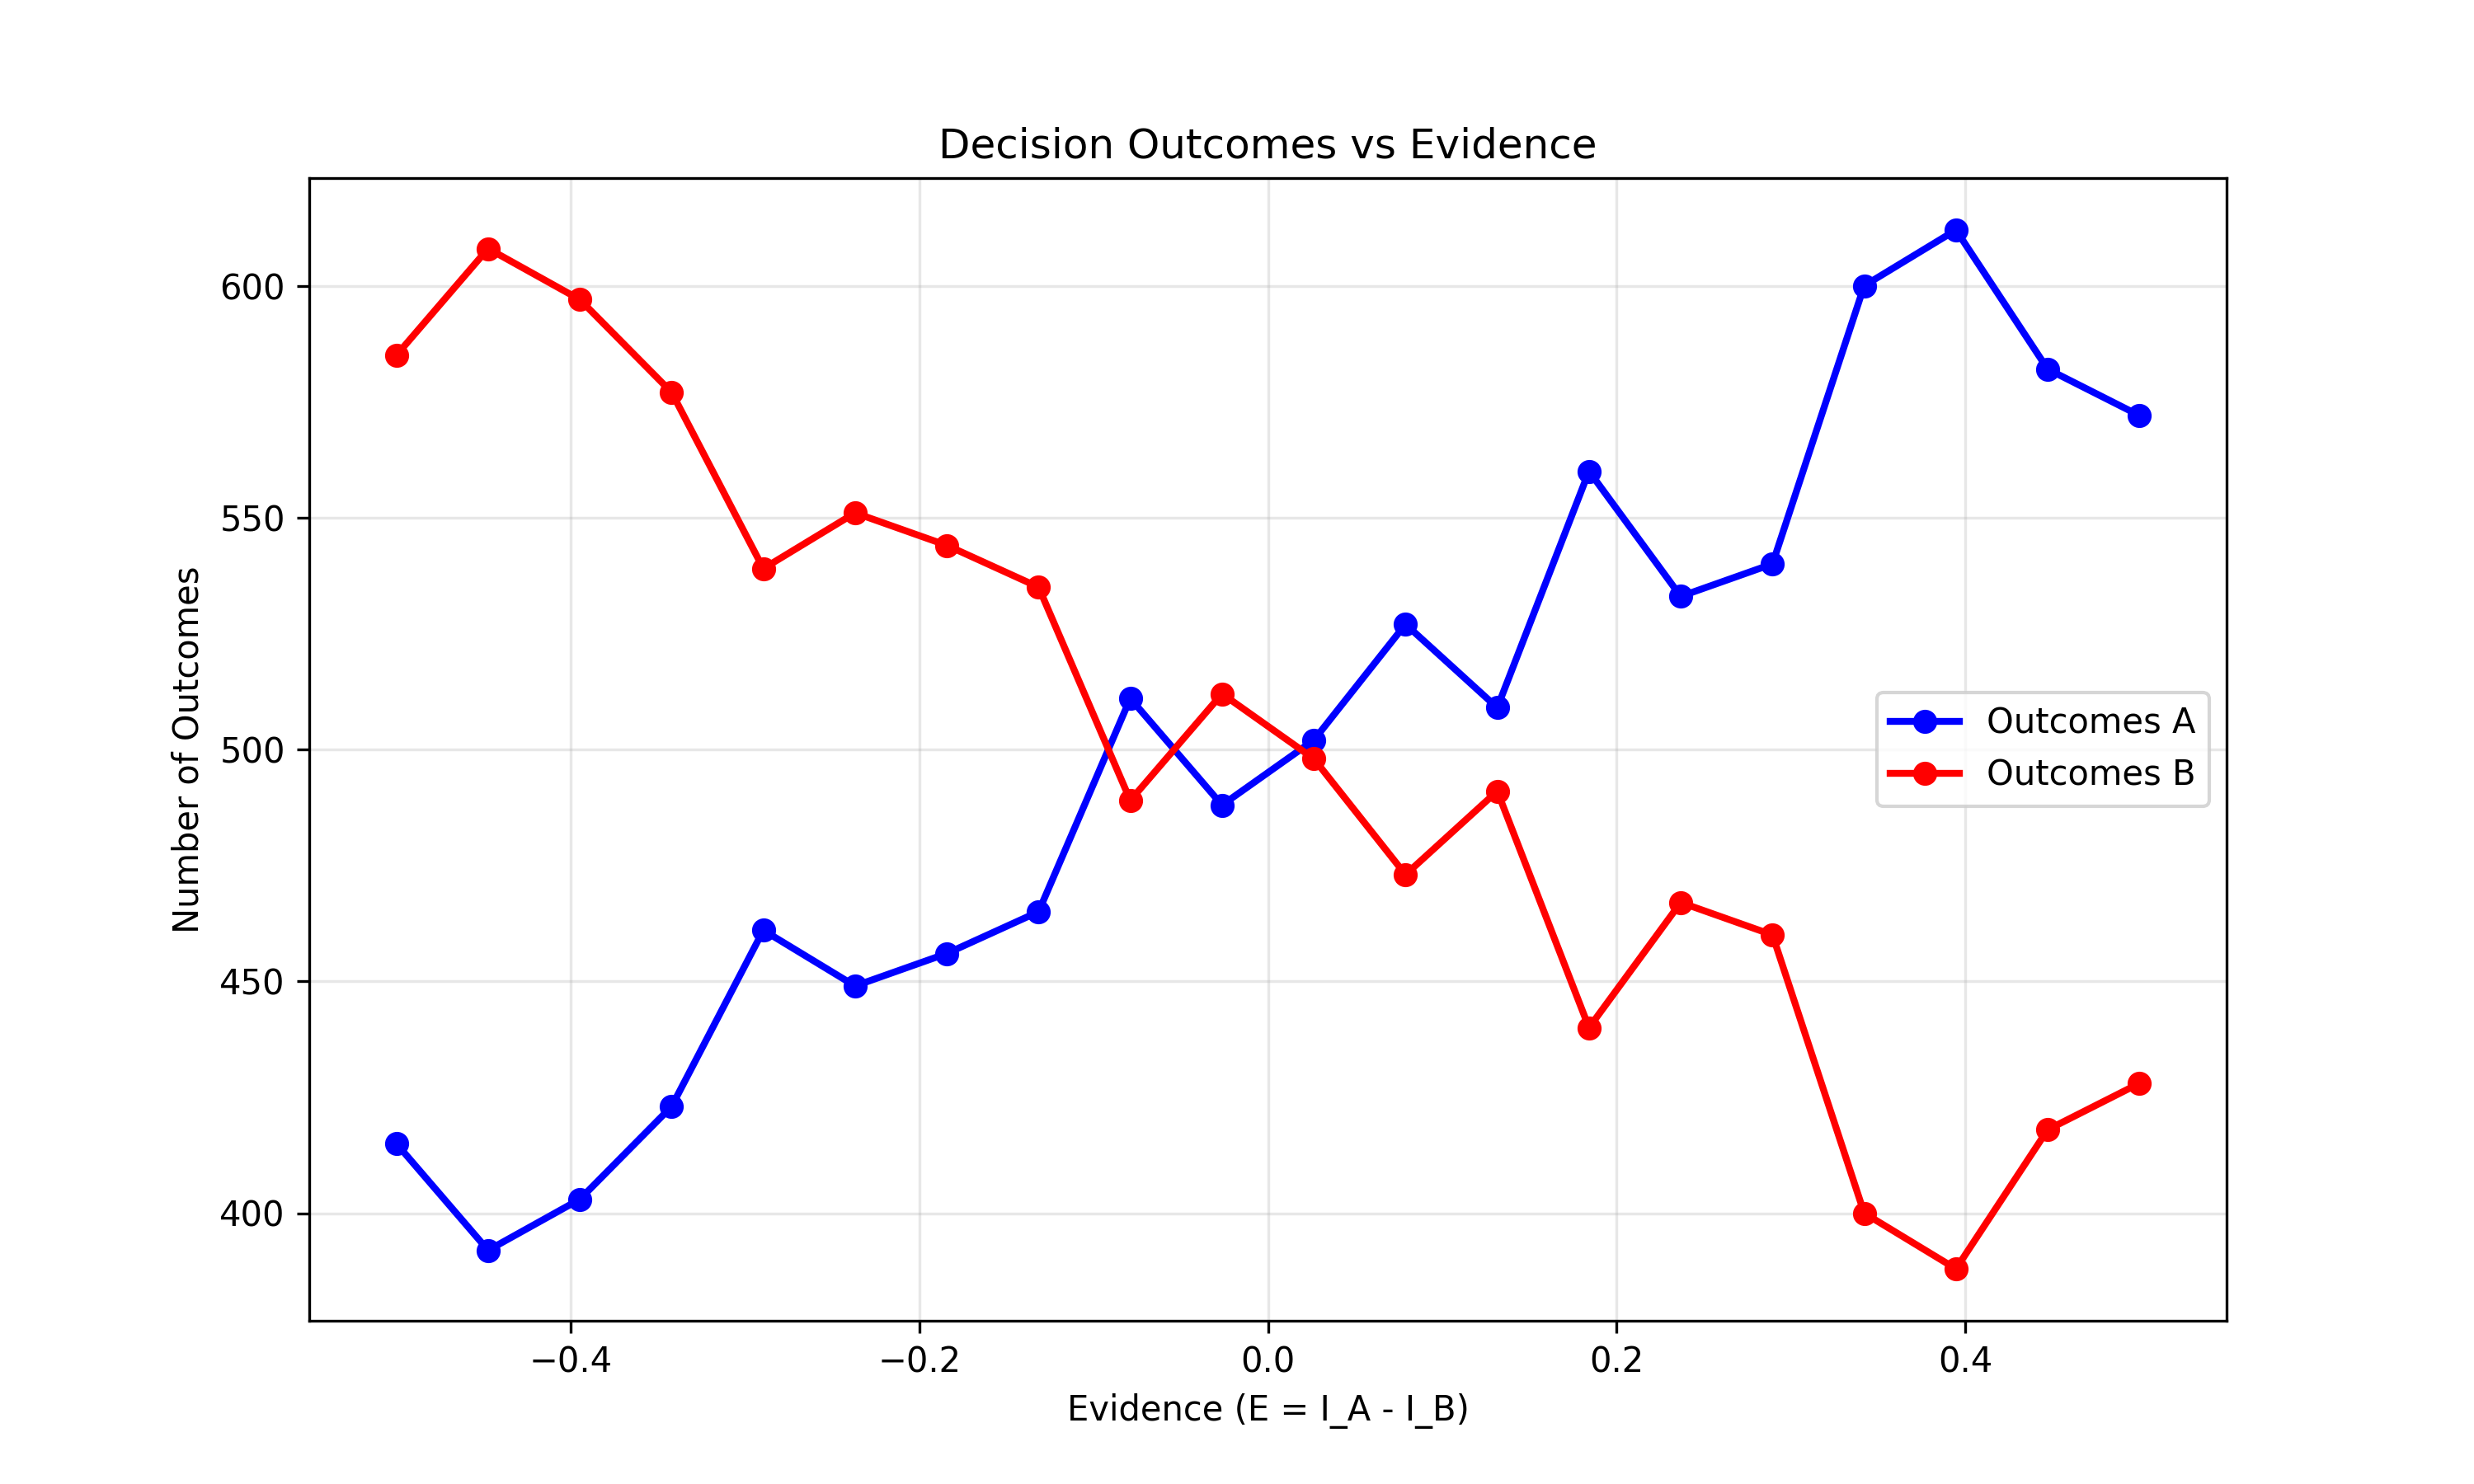
\includegraphics[width=0.6\textwidth]{ddm_evidence_variation.png}
    \caption{Effect of evidence strength $E = I_A - I_B$ on decision outcomes. Positive evidence favors decision A, while negative evidence favors decision B. The transition is smooth and approximately sigmoidal.}
    \label{fig:evidence_variation}
\end{figure}

The evidence variation analysis demonstrates strong relationship between evidence direction and decision bias, 
 and it depicts a symmetric response around $E = 0$ (no bias condition) and a transition between decision preferences. 
Additionally, evidence strength determines the steepness of the preference transition.

\subsection{Reaction times distributions}

We analyzed reaction time distributions for three different evidence levels: $E = 0$, $E = 0.01$, and $E = 0.05$, using parameters $I_B = 1.0$, $\sigma = 7$, and $\mu = 20$.

% FIGURE PLACEHOLDER FOR REACTION TIME DISTRIBUTIONS
\begin{figure}[H]
    \centering
    % INSERT YOUR COMBINED REACTION TIME PLOT HERE
    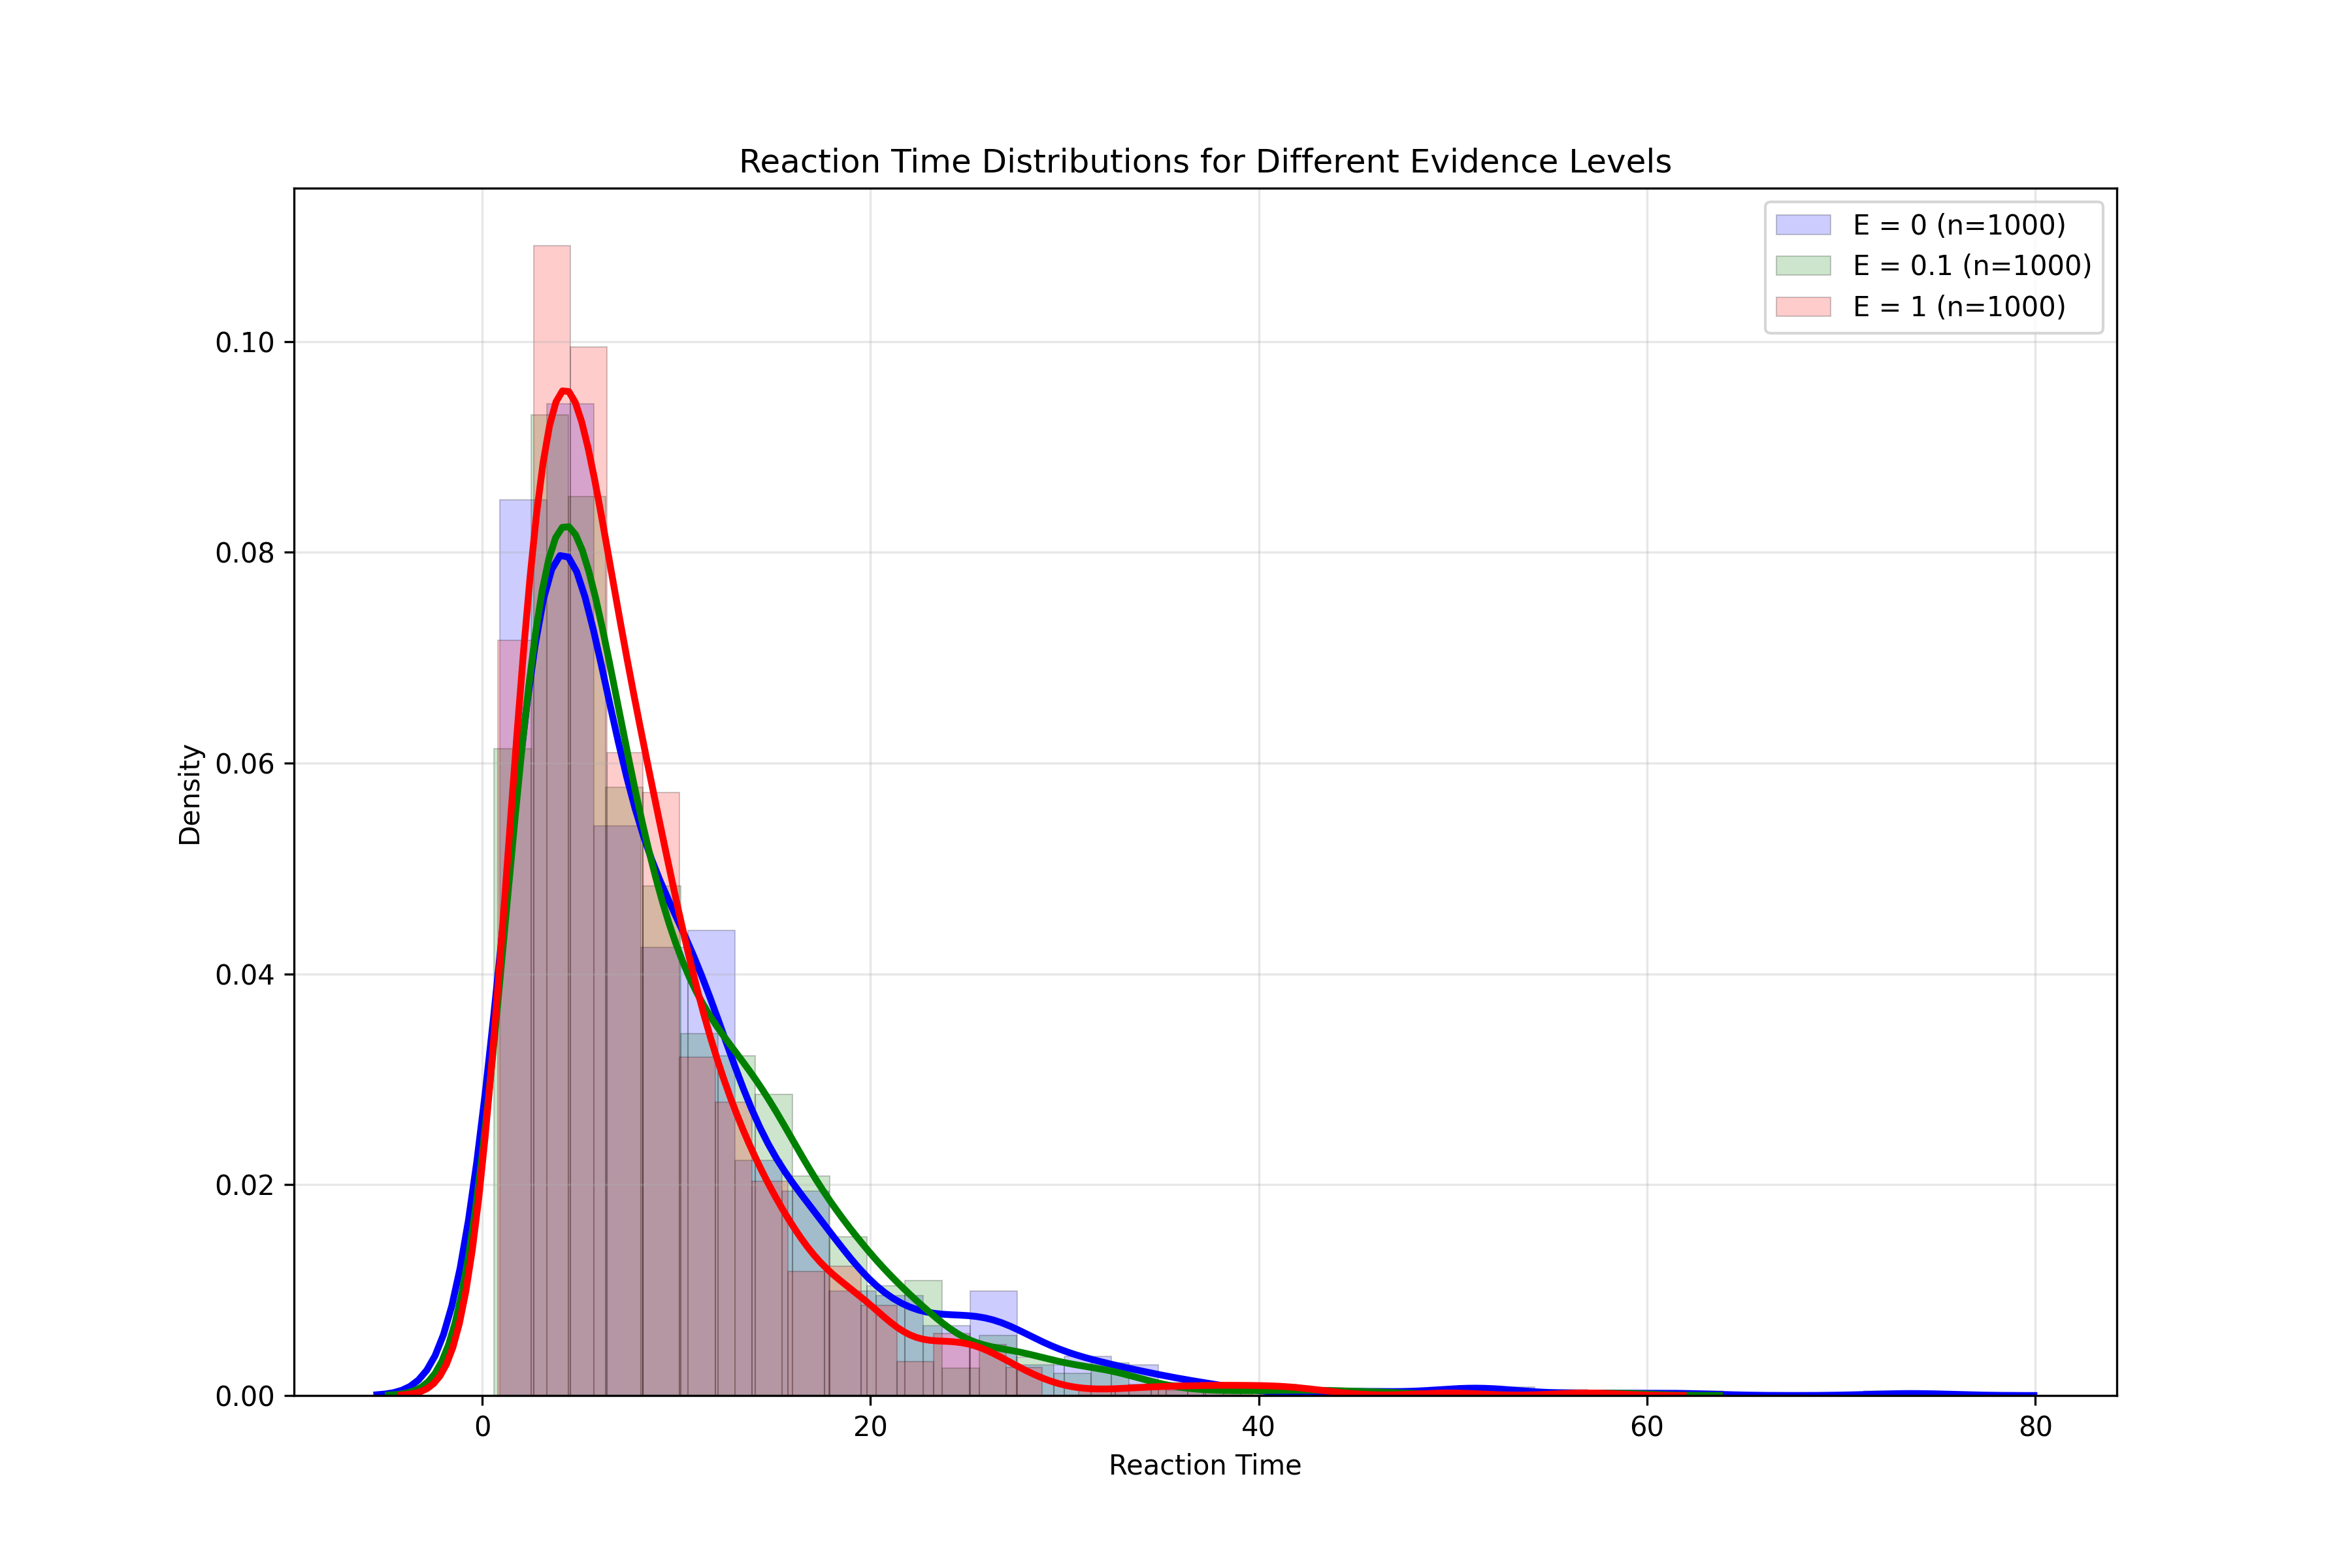
\includegraphics[width=0.6\textwidth]{ddm_combined_reaction_times.png}
    \caption{Reaction time distributions for different evidence levels. The distributions show how evidence strength affects both the speed and variability of decision-making.}
    \label{fig:reaction_times}
\end{figure}

% TABLE FOR REACTION TIME STATISTICS - Fill in your actual values
\begin{table}[H]
    \centering
    \begin{tabular}{@{}lccc@{}}
        \toprule
        Evidence (E) & Mean RT & Std RT \\
        \midrule
        0.0 & 9.52 & 8.39 \\
        0.1 & 9.18 & 7.21 \\
        1.0 & 8.14 & 6.58 \\
        5.0 & 4.27 & 2.79 \\
        \bottomrule
    \end{tabular}
    \caption{Reaction time statistics for different evidence levels. RT = Reaction Time.}
    \label{tab:reaction_times}
\end{table}

The reaction time analysis reveals several key findings. Higher evidence levels lead to significantly faster mean reaction times, while simultaneously reducing reaction time variability (lower standard deviation). Stronger evidence also increases the proportion of trials reaching a decision within the time limit. The reaction time distributions consistently show positive skew, which aligns with empirical findings in perceptual decision-making literature. These results demonstrate how evidence strength directly influences both the speed and consistency of the decision-making process.

% \section{Discussion}

% \subsection{Biological Interpretation}

% The drift-diffusion model provides a biologically plausible account of neural decision-making processes. The decision variable $x(t)$ can be interpreted as the difference in firing rates between neural populations encoding the two alternatives. The drift term $(I_A - I_B)$ represents the quality of sensory evidence, while the noise term $\sigma\eta(t)$ captures the inherent variability in neural responses.

% \subsection{Parameter Significance}

% \subsubsection{Decision Threshold ($\mu$)}
% The decision threshold represents the amount of evidence required before committing to a choice. Neurobiologically, this could correspond to the activation level needed for motor preparation areas to initiate a response. Higher thresholds implement a more conservative decision strategy, trading speed for accuracy.

% \subsubsection{Evidence Strength ($E = I_A - I_B$)}
% Evidence strength captures the quality or reliability of sensory information favoring each alternative. In visual motion discrimination tasks, this would correspond to the coherence level of moving dots. The sigmoidal relationship between evidence and choice probability is a hallmark of perceptual decision-making.

% \subsubsection{Noise Magnitude ($\sigma$)}
% Neural noise reflects the stochastic nature of neural firing and represents internal uncertainty in the decision process. Higher noise levels increase decision variability and can lead to suboptimal choices even with clear evidence.

% \subsection{Implications for Neuroscience}

% The drift-diffusion model successfully captures several key phenomena observed in behavioral and neurophysiological studies:

% \begin{itemize}
%     \item The speed-accuracy trade-off mediated by decision thresholds
%     \item The relationship between stimulus strength and reaction time
%     \item The characteristic shapes of reaction time distributions
%     \item The neural correlates of evidence accumulation in areas like the lateral intraparietal area (LIP)
% \end{itemize}

% \subsection{Model Limitations}

% While powerful, the drift-diffusion model makes several simplifying assumptions:

% \begin{itemize}
%     \item Constant drift rate (evidence strength doesn't vary over time)
%     \item Stationary noise characteristics
%     \item Perfect evidence integration (no leakage or decay)
%     \item Symmetric decision bounds
% \end{itemize}

% Extensions of the model address some of these limitations, including time-varying drift rates, asymmetric bounds, and evidence decay mechanisms.

\section{Conclusions}

This computational analysis of the drift-diffusion model demonstrates its effectiveness in capturing fundamental aspects of perceptual decision-making. Key findings include: (1) the model successfully reproduces the stochastic nature of decision processes (Fig 1); (2) decision thresholds create a speed-accuracy trade-off, with higher thresholds leading to more accurate but slower decisions due to higher evidence requirements and lower variance (Fig 2); (3) evidence strength directly influences both choice bias and reaction time characteristics (Fig 3); and (4) reaction time distributions show the expected positive skew and systematic variation with evidence strength (Fig 4).

The drift-diffusion model remains a cornerstone framework for understanding decision-making in neuroscience, providing quantitative predictions that can be tested against behavioral and neural data. Its simplicity and mathematical tractability make it an excellent starting point for more complex models of cognitive processes.

% Future work could extend this analysis to include:
% \begin{itemize}
%     \item Time-varying evidence and adaptive decision bounds
%     \item Multi-alternative decision scenarios
%     \item Integration with neural network models for more biologically realistic implementations
%     \item Comparison with alternative decision-making frameworks
% \end{itemize}

% \section*{Acknowledgments}

% This work was completed as part of the Methods in Computational Neuroscience course. The Python implementation utilized object-oriented programming principles to create a flexible framework for drift-diffusion model analysis.

% \bibliographystyle{plain}
% % Add your references here if needed
% % \bibliography{references}

\end{document}